%%%%%%%%%%%%%%%%%%%%%%%%%%%%%%%%%%%%%%%%%%%%%%%%%%%%%%%%%%%%%%%%%%%%%%%%%%%

\documentclass{standalone}

\usepackage{amsmath}
\usepackage{mathptmx}
\usepackage{pgfplots}
\usetikzlibrary{external}
\tikzexternalize{sin-cos}
\pgfplotsset{compat=1.16}

%% IEEE uses Times Roman font, so we'll default to Times.
%% These three commands make up the entire times.sty package.
\renewcommand{\rmdefault}{ptm}
\renewcommand{\ttdefault}{pcr}
\normalfont\selectfont

\begin{document}

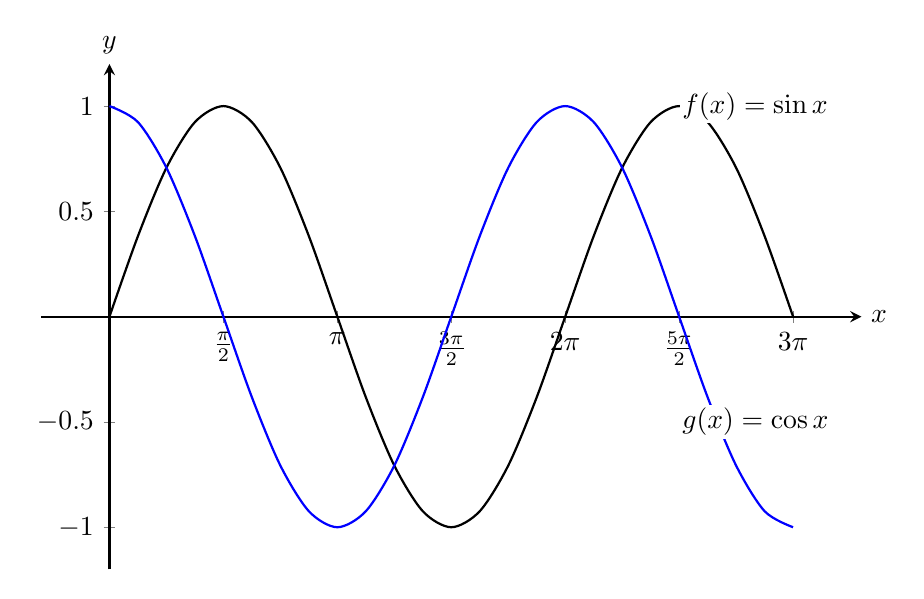
\begin{tikzpicture}
\tikzset{%%
  every mark/.append style={scale=1.0},%%
  scale=1.0%%
}
\pgfplotsset{%%
  every axis/.append style={font=\normalsize}%%
}

\begin{axis}[%%
  axis line style=thick,%%
  axis lines=center,%%
  enlargelimits=true,%%
  height=8cm,%%
  plotStyle/.style={%%
    domain=0:3*pi,%%
    mark=none,%%
    smooth,%%
    thick%%
  },%%
  width=12cm,%%
  %%
  %% x-axis
  xlabel={\normalsize $x$},%%
  xlabel style=right,%%
  xtick={%%
    0, 1.570796,3.141592,4.712388,6.283185,7.853982,9.424778%%
  },%%
  xticklabels={%%
    0,$\frac{\pi}{2}$,$\pi$,$\frac{3\pi}{2}$,$2\pi$,$\frac{5\pi}{2}$,$3\pi$%%
  },%%
  %%
  %% y-axis
  ylabel={\normalsize $y$},%%
  ylabel style=above%%
]
%%
%%
%% The sine function f(x) = sin(x).
\addplot+ [plotStyle,black]
{sin(deg(x))};
\node[fill=white,inner sep=1pt,right] at (7.8539,1) {$f(x) = \sin x$};
%%
%%
%% The cosine function g(x) = cos(x).
\addplot+ [plotStyle,blue]
{cos(deg(x))};
\node[fill=white,inner sep=1pt,right] at (7.8539,-0.5) {$g(x) = \cos x$};
\end{axis}
\end{tikzpicture}

\end{document}
